\documentclass[
	classe=$2^{de}$
]{évaluation}

\usepackage{tcolorbox}
\usetikzlibrary{calc}

\newcounter{LetterCounter}

\author{}
\date{}

\begin{document}

\title{Évaluation : Vecteurs (Sujet A)}
\maketitle

\begin{tcolorbox}
	La calculatrice est autorisée.

	Les exercices 5 et 6 sont à faire sur une feuille à part.
\end{tcolorbox}

% 3 points ?
\begin{exercice}
	\begin{enumerate}
		\item Deux vecteurs sont égaux si ils ont la même \correctionDots{direction}, le même \correctionDots{sens} et la

		      même \correctionDots{norme}.
		\item Si deux vecteurs ont la même direction, la même norme mais des sens opposés, alors ils sont

		      \correctionDots{opposés}.
		\item \

		      \begin{minipage}{0.7\linewidth}
			      En se basant sur la figure ci-contre, répondre VRAI ou FAUX

			      à chaque question :
		      \end{minipage}
		      \begin{minipage}{0.25\linewidth}
			      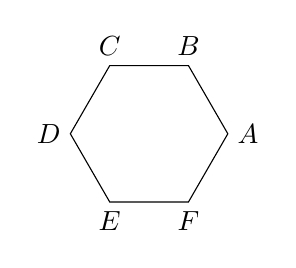
\begin{tikzpicture}
				      \coordinate (O) at (0,0);
				      \coordinate (A) at (1,0);
				      \coordinate[rotate around={60:(O)}] (B) at (A);
				      \coordinate[rotate around={60:(O)}] (C) at (B);
				      \coordinate[rotate around={60:(O)}] (D) at (C);
				      \coordinate[rotate around={60:(O)}] (E) at (D);
				      \coordinate[rotate around={60:(O)}] (F) at (E);
				      \draw (A) -- (B) -- (C) -- (D) -- (E) -- (F) -- cycle;
				      \node[right] at (A) {$A$};
				      \node[above] at (B) {$B$};
				      \node[above] at (C) {$C$};
				      \node[left] at (D) {$D$};
				      \node[below] at (E) {$E$};
				      \node[below] at (F) {$F$};
			      \end{tikzpicture}
		      \end{minipage}
		      \begin{multicols}{2}
			      \begin{enumerate}
				      \item $\vec{AB} = \vec{ED}$ : \correctionDots{VRAI}
				      \item $\vec{DA} = \vec{CB}$ : \correctionDots{FAUX}
				      \item $\vec{DB}$ et $\vec{AE}$ ont la même direction : \correctionDots{VRAI}
				      \item $\vec{CF}$ et $\vec{EB}$ ont la même norme : \correctionDots{VRAI}
			      \end{enumerate}
		      \end{multicols}
	\end{enumerate}
\end{exercice}

% 4-6 points
\begin{exercice}
	\begin{center}
		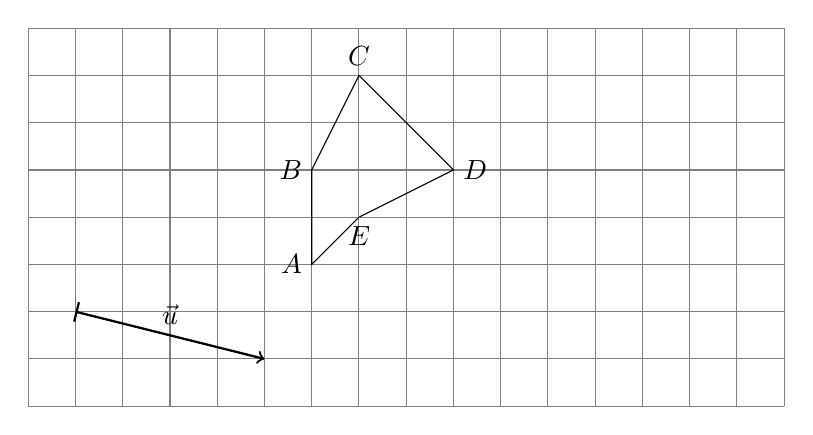
\begin{tikzpicture}[scale=0.6]
			\draw[thin,gray] (0,0) grid (16,8);

			\coordinate (A) at (6,3);
			\coordinate (B) at ($(A) + (0,2)$);
			\coordinate (C) at ($(B) + (1,2)$);
			\coordinate (D) at ($(C) + (2,-2)$);
			\coordinate (E) at ($(D) + (-2,-1)$);

			\draw (A) -- (B) -- (C) -- (D) -- (E) -- cycle;
			\foreach \p/\dir in {A/left,B/left,C/above,D/right,E/below} {
					\node[\dir] at (\p) {$\p$};
				}

			\coordinate (VecU) at (4,-1);
			\coordinate (Vec2) at ($(B) - (D) + (A) - (E)$);

			\draw[thick,|->] (1,2) -- node[above] {$\vec{u}$} ++(VecU);

			\ifdefined\makeCorrection
				\draw[red] ($(A) + (VecU)$) -- ($(B) + (VecU)$) -- ($(C) + (VecU)$) -- ($(D) + (VecU)$) -- ($(E) + (VecU)$) -- cycle;
				\draw[red] ($(A) + (Vec2)$) -- ($(B) + (Vec2)$) -- ($(C) + (Vec2)$) -- ($(D) + (Vec2)$) -- ($(E) + (Vec2)$) -- cycle;
			\fi
		\end{tikzpicture}
	\end{center}

	\begin{enumerate}
		\item Construire le translaté de la figure ABCDE par le vecteur $\vec{u}$.
		\item Construire le translaté de la figure ABCDE par le vecteur $\vec{CB} + \vec{DC} + \vec{EA}$.
	\end{enumerate}
\end{exercice}

\begin{exercice}
	\begin{center}
		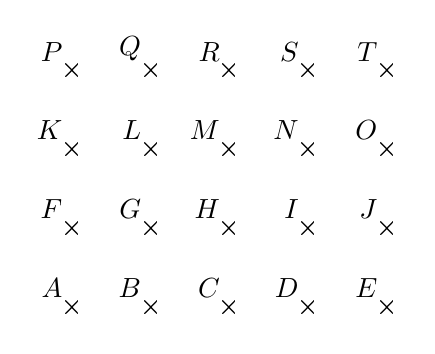
\begin{tikzpicture}
			\setcounter{LetterCounter}{0}
			\foreach \y in {0,...,3} {
					\foreach \x in {0,...,4} {
							\stepcounter{LetterCounter}
							\coordinate (\Alph{LetterCounter}) at (\x,\y);
							\node at (\Alph{LetterCounter}) {×};
							\node[above left] at (\Alph{LetterCounter}) {$\Alph{LetterCounter}$};
						}
				}
		\end{tikzpicture}
	\end{center}
	Pour chaque vecteur ci-dessous, donner \textbf{deux} de ses représentants :
	\begin{enumerate}
		\item $\vec{AB} + \vec{BG}$ : \correction{$\vec{AG}$ et $\vec{FL}$}
		\item $\frac{1}{4}\vec{FJ}$ : \correction{$\vec{FG}$ et $\vec{KL}$}
		\item $2\vec{KM} - \vec{EI}$ : \correction{$\vec{KS}$ et $\vec{FN}$}
		\item $2\vec{FR} + \frac{2}{3}\vec{RC}$ : \correction{$\vec{FT}$ et $\vec{AO}$}
	\end{enumerate}
\end{exercice}

\newpage

\begin{exercice}
	\begin{center}
		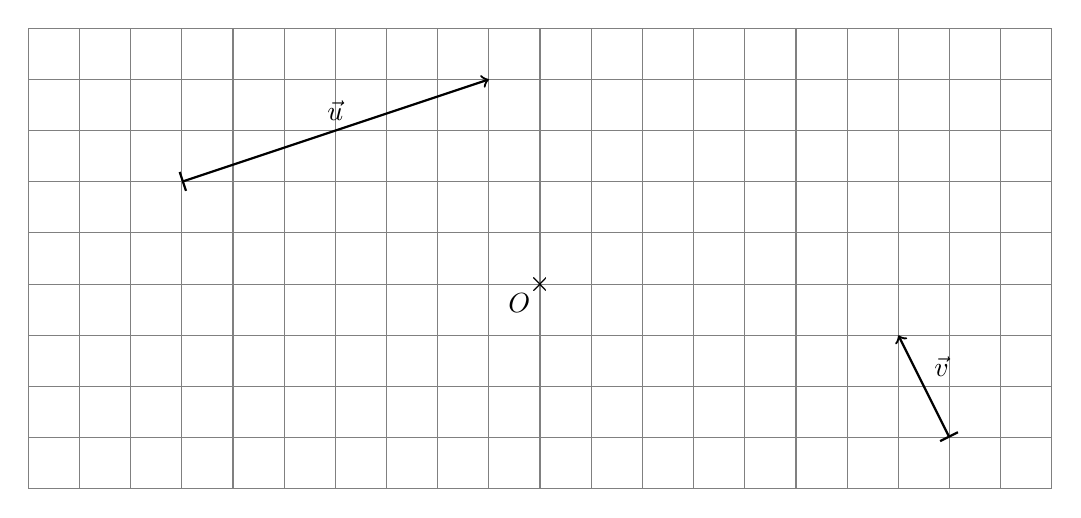
\begin{tikzpicture}[scale=0.65]
			\draw[thin,gray] (0,0) grid (20,9);

			\coordinate (O) at (10,4);
			\coordinate (VecU) at (6,2);
			\coordinate (StartVecU) at (3,6);
			\coordinate (VecV) at (-1,2);
			\coordinate (StartVecV) at (18,1);

			\node at (O) {×};
			\node[below left] at (O) {$O$};
			\draw[thick,|->] (StartVecU) -- node[above] {$\vec{u}$} ++(VecU);
			\draw[thick,|->] (StartVecV) -- node[above right] {$\vec{v}$} ++(VecV);

			\ifdefined\makeCorrection
				\coordinate (Vec1) at ($(VecU) + (VecV)$);
				\coordinate (Vec2) at ($-1*(VecU) + 2*(VecV)$);
				\coordinate (Vec3) at ($0.5*(VecU) - (VecV)$);

				\draw[red,thick,|->] (O) -- node[left] {$\vec{u} + \vec{v}$} ++(Vec1);
				\draw[red,thick,|->] (O) -- node[above] {$-\vec{u} + 2\vec{v}$} ++(Vec2);
				\draw[red,thick,|->] (O) -- node[above] {$\frac{1}{2}\vec{u} - \vec{v}$} ++(Vec3);
			\fi
		\end{tikzpicture}
	\end{center}

	\begin{enumerate}
		\item Tracer le représentant du vecteur $\vec{u} + \vec{v}$ ayant pour origine $O$.
		\item Tracer le représentant du vecteur $-\vec{u} + 2\vec{v}$ ayant pour origine $O$.
		\item Tracer le représentant du vecteur $\frac{1}{2}\vec{u} - \vec{v}$ ayant pour origine $O$.
	\end{enumerate}
\end{exercice}

\begin{exercice}(À faire sur une feuille à part)

	Simplifier les expressions suivantes, en détaillant les calculs :
	\begin{enumerate}
		\item $\vec{AC} + \vec{CD} + \vec{DE}$ \correction{$ = \vec{AE}$}
		\item $\vec{FE} - \vec{CD} + \vec{ED}$ \correction{$ = \vec{FC}$}
		\item $\vec{EA} - (\vec{EC} + \vec{ED}) + \vec{AD}$ \correction{$ = \vec{CE}$}
		\item $\vec{AE} + \vec{TA} + \vec{FT} + \vec{EF}$ \correction{$ = \vec{0}$}
		\item $5(\vec{u} + \vec{v}) - 2\vec{v}$ \correction{$ = 5\vec{u} + 3\vec{v}$}
	\end{enumerate}
\end{exercice}

\begin{exercice}(À faire sur une feuille à part)

	Soit $ABC$ un triangle quelconque. Les points $K$ et $L$ vérifient : $\vec{AK} = 3\vec{AB}$ et $\vec{AL} = 3\vec{AC}$.
	\begin{enumerate}
		\item Faire une figure représentant cette situation.
		\item (Les étapes de cette question doivent être bien détaillées) En remarquant que $\vec{KL} = \vec{KA} + \vec{AL}$, montrer que $\vec{KL} = 3\vec{BC}$.
	\end{enumerate}

	\ifdefined\makeCorrection
		\begin{center}
			\begin{tikzpicture}
				\coordinate (A) at (0,1);
				\coordinate (B) at (1,2);
				\coordinate (C) at (3,1);
				\coordinate (K) at ($(A) + 3*(B) - 3*(A)$);
				\coordinate (L) at ($(A) + 3*(C) - 3*(A)$);

				\draw[red]
				(A) node[left] {$A$} --
				(B) node[above] {$B$} --
				(C) node[right] {$C$} --
				cycle;
				\node[red] at (K) {×};
				\node[red] at (L) {×};
				\node[red,above] at (K) {$K$};
				\node[red,above] at (L) {$L$};
			\end{tikzpicture}
		\end{center}

		{\color{red}
		On a alors
		\begin{align*}
			\vec{KL} & = \vec{KA} + \vec{AL}    \\
			         & = -\vec{AK} + \vec{AL}   \\
			         & = -3\vec{AB} + 3\vec{AC} \\
			         & = 3\vec{BA} + 3\vec{AC}  \\
			         & = 3(\vec{BA} + \vec{AC}) \\
			         & = 3\vec{BC}
		\end{align*}
		}
	\fi
\end{exercice}

%%%%%%%%%%%%%%%%%%%%%%%%%%%
% SUJET B                 %
%%%%%%%%%%%%%%%%%%%%%%%%%%%

\setcounter{exercice}{1}
\newpage

\title{Évaluation : Vecteurs (Sujet B)}
\maketitle

\begin{tcolorbox}
	La calculatrice est autorisée.

	Les exercices 5 et 6 sont à faire sur une feuille à part.
\end{tcolorbox}

% 3 points ?
\begin{exercice}
	\begin{enumerate}
		\item Deux vecteurs sont égaux si ils ont la même \correctionDots{direction}, le même \correctionDots{sens} et la

		      même \correctionDots{norme}.
		\item Si deux vecteurs ont la même direction, la même norme mais des sens opposés, alors ils sont

		      \correctionDots{opposés}.
		\item \

		      \begin{minipage}{0.7\linewidth}
			      En se basant sur la figure ci-contre, répondre VRAI ou FAUX

			      à chaque question :
		      \end{minipage}
		      \begin{minipage}{0.25\linewidth}
			      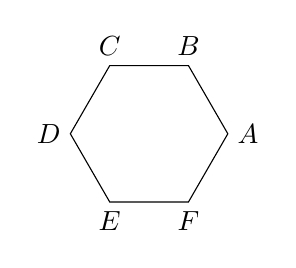
\begin{tikzpicture}
				      \coordinate (O) at (0,0);
				      \coordinate (A) at (1,0);
				      \coordinate[rotate around={60:(O)}] (B) at (A);
				      \coordinate[rotate around={60:(O)}] (C) at (B);
				      \coordinate[rotate around={60:(O)}] (D) at (C);
				      \coordinate[rotate around={60:(O)}] (E) at (D);
				      \coordinate[rotate around={60:(O)}] (F) at (E);
				      \draw (A) -- (B) -- (C) -- (D) -- (E) -- (F) -- cycle;
				      \node[right] at (A) {$A$};
				      \node[above] at (B) {$B$};
				      \node[above] at (C) {$C$};
				      \node[left] at (D) {$D$};
				      \node[below] at (E) {$E$};
				      \node[below] at (F) {$F$};
			      \end{tikzpicture}
		      \end{minipage}
		      \begin{multicols}{2}
			      \begin{enumerate}
				      \item $\vec{AB} = \vec{ED}$ : \correctionDots{VRAI}
				      \item $\vec{DA} = \vec{CB}$ : \correctionDots{FAUX}
				      \item $\vec{DB}$ et $\vec{AE}$ ont la même direction : \correctionDots{VRAI}
				      \item $\vec{CF}$ et $\vec{EB}$ ont la même norme : \correctionDots{VRAI}
			      \end{enumerate}
		      \end{multicols}
	\end{enumerate}
\end{exercice}

% 4-6 points
\begin{exercice}
	\begin{center}
		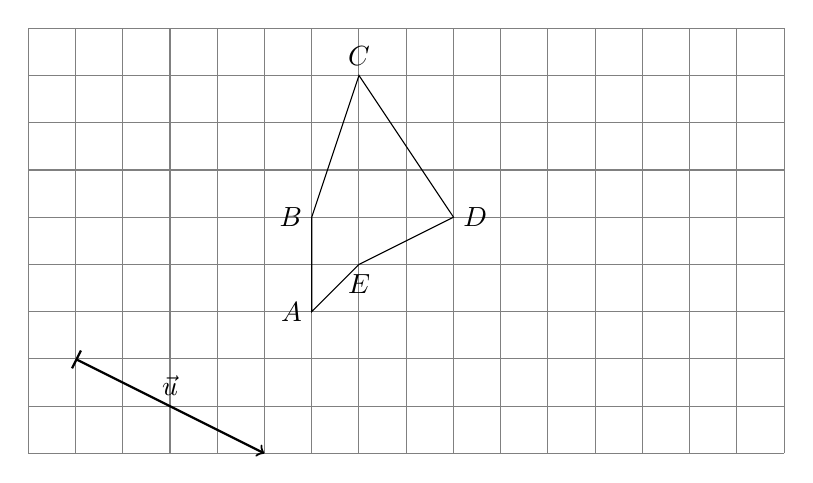
\begin{tikzpicture}[scale=0.6]
			\draw[thin,gray] (0,0) grid (16,9);

			\coordinate (A) at (6,3);
			\coordinate (B) at ($(A) + (0,2)$);
			\coordinate (C) at ($(B) + (1,3)$);
			\coordinate (D) at ($(C) + (2,-3)$);
			\coordinate (E) at ($(D) + (-2,-1)$);

			\draw (A) -- (B) -- (C) -- (D) -- (E) -- cycle;
			\foreach \p/\dir in {A/left,B/left,C/above,D/right,E/below} {
					\node[\dir] at (\p) {$\p$};
				}

			\coordinate (VecU) at (4,-2);
			\coordinate (Vec2) at ($(B) - (D) + (A) - (E)$);

			\draw[thick,|->] (1,2) -- node[above] {$\vec{u}$} ++(VecU);

			\ifdefined\makeCorrection
				\draw[red] ($(A) + (VecU)$) -- ($(B) + (VecU)$) -- ($(C) + (VecU)$) -- ($(D) + (VecU)$) -- ($(E) + (VecU)$) -- cycle;
				\draw[red] ($(A) + (Vec2)$) -- ($(B) + (Vec2)$) -- ($(C) + (Vec2)$) -- ($(D) + (Vec2)$) -- ($(E) + (Vec2)$) -- cycle;
			\fi
		\end{tikzpicture}
	\end{center}

	\begin{enumerate}
		\item Construire le translaté de la figure ABCDE par le vecteur $\vec{u}$.
		\item Construire le translaté de la figure ABCDE par le vecteur $\vec{CB} + \vec{DC} + \vec{EA}$.
	\end{enumerate}
\end{exercice}

\begin{exercice}
	\begin{center}
		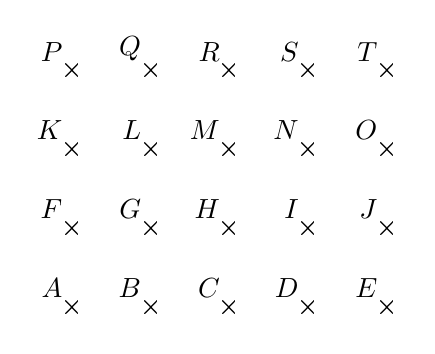
\begin{tikzpicture}
			\setcounter{LetterCounter}{0}
			\foreach \y in {0,...,3} {
					\foreach \x in {0,...,4} {
							\stepcounter{LetterCounter}
							\coordinate (\Alph{LetterCounter}) at (\x,\y);
							\node at (\Alph{LetterCounter}) {×};
							\node[above left] at (\Alph{LetterCounter}) {$\Alph{LetterCounter}$};
						}
				}
		\end{tikzpicture}
	\end{center}
	Pour chaque vecteur ci-dessous, donner \textbf{deux} de ses représentants :
	\begin{enumerate}
		\item $\vec{FG} + \vec{GL}$ : \correction{$\vec{AG}$ et $\vec{FL}$}
		\item $\frac{1}{2}\vec{KO}$ : \correction{$\vec{KM}$ et $\vec{LN}$}
		\item $2\vec{AH} - \vec{IE}$ : \correction{$\vec{AS}$ et $\vec{BT}$}
		\item $2\vec{TH} + \frac{2}{3}\vec{CR}$ : \correction{$\vec{TF}$ et $\vec{OA}$}
	\end{enumerate}
\end{exercice}

\newpage

\begin{exercice}
	\begin{center}
		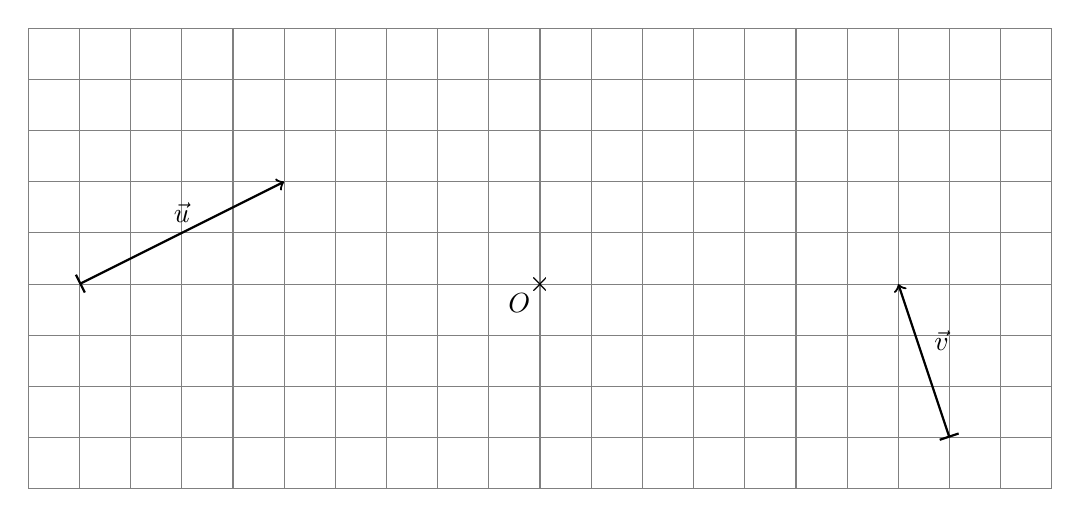
\begin{tikzpicture}[scale=0.65]
			\draw[thin,gray] (0,0) grid (20,9);

			\coordinate (O) at (10,4);
			\coordinate (VecU) at (4,2);
			\coordinate (StartVecU) at (1,4);
			\coordinate (VecV) at (-1,3);
			\coordinate (StartVecV) at (18,1);

			\node at (O) {×};
			\node[below left] at (O) {$O$};
			\draw[thick,|->] (StartVecU) -- node[above] {$\vec{u}$} ++(VecU);
			\draw[thick,|->] (StartVecV) -- node[above right] {$\vec{v}$} ++(VecV);

			\ifdefined\makeCorrection
				\coordinate (Vec1) at ($(VecU) + (VecV)$);
				\coordinate (Vec2) at ($-1*(VecU) + 2*(VecV)$);
				\coordinate (Vec3) at ($0.5*(VecU) - (VecV)$);

				\draw[red,thick,|->] (O) -- node[left] {$\vec{u} + \vec{v}$} ++(Vec1);
				\draw[red,thick,|->] (O) -- node[above] {$-\vec{u} + 2\vec{v}$} ++(Vec2);
				\draw[red,thick,|->] (O) -- node[above] {$\frac{1}{2}\vec{u} - \vec{v}$} ++(Vec3);
			\fi
		\end{tikzpicture}
	\end{center}

	\begin{enumerate}
		\item Tracer le représentant du vecteur $\vec{u} + \vec{v}$ ayant pour origine $O$.
		\item Tracer le représentant du vecteur $-\vec{u} + 2\vec{v}$ ayant pour origine $O$.
		\item Tracer le représentant du vecteur $\frac{1}{2}\vec{u} - \vec{v}$ ayant pour origine $O$.
	\end{enumerate}
\end{exercice}

\begin{exercice}(À faire sur une feuille à part)

	Simplifier les expressions suivantes, en détaillant les calculs :
	\begin{enumerate}
		\item $\vec{FC} + \vec{CD} + \vec{DE}$ \correction{$ = \vec{FE}$}
		\item $\vec{AE} - \vec{CD} + \vec{ED}$ \correction{$ = \vec{AC}$}
		\item $\vec{FB} - (\vec{FD} + \vec{FE}) + \vec{BE}$ \correction{$ = \vec{DF}$}
		\item $\vec{BE} + \vec{TB} + \vec{FT} + \vec{EF}$ \correction{$ = \vec{0}$}
		\item $7(\vec{u} + \vec{v}) - 3\vec{v}$ \correction{$ = 7\vec{u} + 4\vec{v}$}
	\end{enumerate}
\end{exercice}

\begin{exercice}(À faire sur une feuille à part)

	Soit $ABC$ un triangle quelconque. Les points $K$ et $L$ vérifient : $\vec{AK} = 3\vec{AB}$ et $\vec{AL} = 3\vec{AC}$.
	\begin{enumerate}
		\item Faire une figure représentant cette situation.
		\item (Les étapes de cette question doivent être bien détaillées) En remarquant que $\vec{KL} = \vec{KA} + \vec{AL}$, montrer que $\vec{KL} = 3\vec{BC}$.
	\end{enumerate}

	\ifdefined\makeCorrection
		\begin{center}
			\begin{tikzpicture}
				\coordinate (A) at (0,1);
				\coordinate (B) at (1,2);
				\coordinate (C) at (3,1);
				\coordinate (K) at ($(A) + 3*(B) - 3*(A)$);
				\coordinate (L) at ($(A) + 3*(C) - 3*(A)$);

				\draw[red]
				(A) node[left] {$A$} --
				(B) node[above] {$B$} --
				(C) node[right] {$C$} --
				cycle;
				\node[red] at (K) {×};
				\node[red] at (L) {×};
				\node[red,above] at (K) {$K$};
				\node[red,above] at (L) {$L$};
			\end{tikzpicture}
		\end{center}

		{\color{red}
		On a alors
		\begin{align*}
			\vec{KL} & = \vec{KA} + \vec{AL}    \\
			         & = -\vec{AK} + \vec{AL}   \\
			         & = -3\vec{AB} + 3\vec{AC} \\
			         & = 3\vec{BA} + 3\vec{AC}  \\
			         & = 3(\vec{BA} + \vec{AC}) \\
			         & = 3\vec{BC}
		\end{align*}
		}
	\fi
\end{exercice}

\end{document}